\section{微分}\label{zhang_differential}
%\begin{figure}[htp]
%    \centering
 %   \begin{tikzpicture}[>=latex]
      %\draw[-](0,0)--(3,0)--(3,3)--(0,3)--(0,0);
      %\draw[-](2,0)--(2,3);
    %  \draw[-](0,2)--(3,2);
   %   \node at(1,1){$A=x_0^2$};
  %\end{tikzpicture}
 % \end{figure}
  \subsection{定义}
  \begin{center}
    设函数$f(x)$在点$x_0$的一个邻域内有定义。$\vartriangle y=f(x_0+\vartriangle x)-f(x_0)$\\\
    如果$\vartriangle y$可以表示为$\vartriangle y=A\vartriangle x+\circ (\vartriangle x)$其中$A$为与$\vartriangle x$无关的常数\\
    则称$f(x)$在点$x_0$可微,$A\vartriangle x$称为$f(x)$在点$x_0$处的微分。\\
    $\mbox{记作:}dy=A\vartriangle x$
  \end{center}
\begin{figure}[htp]
   \centering
    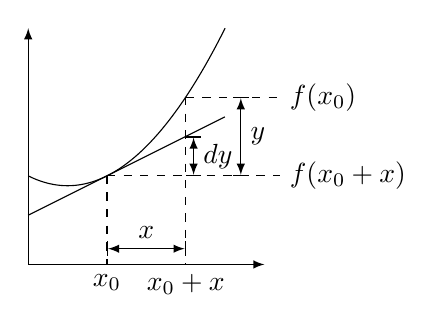
\begin{tikzpicture}[>=latex]
      \draw[->](0,0)--(3,0);
      \draw[->](0,0)--(0,3);
      \draw[domain=0:2.5,samples=1000] plot(\x,{((\x-.5)^2)*(1/2)+1});
      \draw[domain=0:2.5,samples=500] plot(\x,{(\x-1)*(1/2)+9/8});
      \draw[|<->|] (2.1,{(2-1)*(1/2)+9/8})--(2.1,{(((1-.5)^2)*(1/2)+1+(2-1)*(1/2)+9/8)/2})node[right]{$dy$}--(2.1,{((1-.5)^2)*(1/2)+1});
      \draw[dashed](1,{((1-.5)^2)*(1/2)+1})--(1,0)node[below]{$x_0$};
      \draw[dashed](2,{((2-.5)^2)*(1/2)+1})--(2,0)node[below]{$x_0+\vartriangle x$};
     % \node at (3,-1)[below]{常函数\ $f(x)=a\{a\in R\}$};
      \draw[|<->|] (1,.2)--(1.5,.2)node[above]{$\vartriangle x$}--(2,.2);
      \draw[dashed](2,{((2-.5)^2)*(1/2)+1})--(3.2,{((2-.5)^2)*(1/2)+1})node[right]{$f(x_0)$};
      \draw[dashed](1,{((1-.5)^2)*(1/2)+1})--(3.2,{((1-.5)^2)*(1/2)+1})node[right]{$f(x_0+\vartriangle x)$};
      \draw[|<->|](2.7,{((2-.5)^2)*(1/2)+1})--(2.7,{(((2-.5)^2)*(1/2)+1+((1-.5)^2)*(1/2)+1)/2})node[right]{$\vartriangle y$}--(2.7,{((1-.5)^2)*(1/2)+1});
    \end{tikzpicture}
\end{figure}
\begin{align}
    \mbox{可微}\Rightarrow\mbox{可导}\label{differential_to_derivative}\\
    \mbox{可导}\Rightarrow\mbox{可微}\label{derivative_to_differential}
\end{align}

\subsection{微分法则}
\subsubsection{核心根本}
\begin{figure}[htp]
    \centering
    \begin{tikzpicture}[>=latex]
      \draw[->](1.5,.2)--(1.5,.5)--(3,.5)--(3,.2);
      \node at(2.25,.5)[above]{积分};
      \draw[<-](1.5,-.2)--(1.5,-.5)--(3,-.5)--(3,-.2);
      \node at(2.25,-.5)[below]{求导};
      \node at(.5,0){$dy=$};
      \node at(1.5,0){$f'(x)$};
      \node at(2.3,0){$d$};
      \node at(3,0){$x$};
  \end{tikzpicture}
\end{figure}
\subsubsection{四则运算}
\begin{align}
    d\left(u\pm v\right)=du\pm dv\\
    d(uv)=vdu+udv\\
    d\left(\frac{u}{v}\right)=\frac{vdu+udv}{v^2}
\end{align}
\subsubsection{复合运算}
\begin{center}
    $y=f(u),u=g(x)$可微,则$y=f(g(x))$也可微,且
    $$dy=f'(u)du=f'(u)g(x)dx$$
    $u$是否为中间变量都成立,微分的不变性。
\end{center}
\subsubsection{近似计算公式}
$\vartriangle x\rightarrow 0\mbox{时候}dy\approx \vartriangle y$
$$f(x_0+\vartriangle x)-f(x_0)\approx dy=f'(x_0)\vartriangle x$$
$$f(x_0+\vartriangle x)\approx f(x_0)+f'(x_0)\vartriangle x$$